%%%%%%%%%%%%%%%%%  Debut du fichier Latex  %%%%%%%%%%%%%%%%%%%%%%%%%%%%%%
\documentclass[11pt,onecolumn]{article}
%\usepackage[style=numeric,maxnames=1,uniquelist=false]{biblatex}
%\usepackage[backend=bibtex,style=numeric,minnames=4,maxnames=4,firstinits=true,sorting=none]{biblatex} 
\usepackage[backend=bibtex,bibstyle=phys,citestyle=authoryear,maxcitenames=1,minbibnames=3,maxbibnames=3,giveninits=true,natbib,doi=false,isbn=false]{biblatex} 
%\usepackage[authordate,bibencoding=auto,strict,backend=biber,natbib]{biblatex}

 %backend=biber is 'better'  
\makeatletter
\def\blx@maxline{77}
\makeatother
\renewbibmacro{in:}{} % to not have the "In:" to indicate the review
\AtEveryBibitem{\clearfield{title}} % to remove the titles in the biblio
% no page info
\AtEveryBibitem{%
  \ifentrytype{article}{%
    \clearfield{pages}%
  }{%
  }%
}
% no language info
\AtEveryBibitem{\clearlist{language}}
% no language no page
\AtEveryBibitem{%
  \clearfield{volume}%
  \clearfield{number}}
% To avoid parenthesis if no year entry in bib file
\renewbibmacro*{issue+date}{%
  \ifboolexpr{not test {\iffieldundef{year}} or not test {\iffieldundef{issue}}}
    {\printtext[parens]{%
       \iffieldundef{issue}
         {\usebibmacro{date}}
         {\printfield{issue}%
          \setunit*{\addspace}%
          \usebibmacro{date}}}}
    {}%
  \newunit}


\ExecuteBibliographyOptions{isbn=false,url=false,doi=false,eprint=false}

%\bibliography{/Users/Ileyk/Documents/Bibtex/Hubble_fellowship_no_url} 
%\addbibresource{/Users/Ileyk/Documents/Bibtex/CNRS_19_fixed.bib}
\addbibresource{/Users/Ileyk/Work/Job_applications/CNAP_19/CNRS_19_fixed.bib}

%%% Pour un texte en francais


%%\usepackage[applemac]{inputenc}
%\usepackage[francais]{babel}
	         % encodage des lettres accentuees
\usepackage[T1]{fontenc}
\usepackage[utf8]{inputenc}          % encodage des lettres accentuees
%\usepackage{graphicx}
%%\usepackage{graphicx} \def\BIB{}
\usepackage[paper=a4paper,left=2.5cm,right=2.5cm,top=3.5cm,bottom=3.5cm]{geometry}
\usepackage{multicol}
\usepackage{graphicx,wrapfig,lipsum} 
%\def\BIB{}
\usepackage{caption}
\usepackage{subcaption}
\usepackage[pdftex]{hyperref}
%\usepackage{natbib}
\usepackage{url}
\usepackage{perpage} %the perpage package
\MakePerPage{footnote} %the perpage package command
\hypersetup{
    colorlinks,%
    citecolor=blue,%
    filecolor=blue,%
    linkcolor=blue,%
    urlcolor=blue     % can put red here to visualize the links
}

\usepackage{enumitem}
\usepackage{amssymb}

%\renewcommand{\refname}{}

\usepackage{floatrow}

\usepackage{fancyhdr}
\usepackage{lastpage}

\pagestyle{fancy}
\fancyhf{}
\rhead{Research summary}
\lhead{El Mellah Ileyk}
\rfoot{\thepage / \pageref{LastPage}}

\DeclareUnicodeCharacter{00A0}{ }

\usepackage{xspace}

%%% Quelques raccourcis pour la mise en page
\newcommand{\remarque}[1]{{\small \it #1}}
\newcommand{\rubrique}{\bigskip \noindent $\bullet$ }
\newcommand{\sgx}{SgXB\xspace}
\newcommand{\sgxs}{SgXBs\xspace}
\newcommand{\ulx}{ULX\xspace}
\newcommand{\sfxt}{SFXT}
\newcommand{\sg}{Sg\xspace}
\newcommand{\co}{CO\xspace}
\newcommand{\gw}{GW\xspace}
\newcommand{\gws}{GWs\xspace}
\newcommand{\grb}{GRB\xspace}
\newcommand{\grbs}{GRBs\xspace}
\newcommand{\eos}{EOS\xspace}
\newcommand{\mhd}{MHD\xspace}
\newcommand*{\hmxb}{HMXB\@\xspace}
\newcommand*{\hmxbs}{HMXBs\@\xspace}
\newcommand*{\lmxb}{LMXB\@\xspace}
\newcommand*{\rlof}{RLOF\@\xspace}
\newcommand*{\ns}{NS\@\xspace}
\newcommand*{\nss}{NSs\@\xspace}
\newcommand*{\bh}{BH\@\xspace}
\newcommand*{\bhs}{BHs\@\xspace}
\newcommand*{\eg}{e.g.\@\xspace}
\newcommand*{\ie}{i.e.\@\xspace}
\newcommand*{\aka}{a.k.a. \@\xspace}
\newcommand*\diff{\mathop{}\!\mathrm{d}}
\newcommand{\mystar}{{\fontfamily{lmr}\selectfont$\star$}}
\newcommand*{\msun}{$M_{\odot}$\@\xspace}
\newcommand*{\mdotstar}{$\dot{M}_{\text{\mystar}}$\@\xspace}
\newcommand*{\mdotacc}{$\dot{M}_{\text{acc}}$\@\xspace}
\newcommand*{\ledd}{$L_{\text{Edd}}$\@\xspace}


\newcommand{\ignore}[1]{}

%\renewcommand*\rmdefault{iwona}

%\pagenumbering{gobble}

%\bibliographystyle{abbrvnat}
%\setcitestyle{authoryear,open={((},close={))}}

%\renewcommand{\thefootnote}{\roman{footnote}}

% -------------------------------------------------
\newcommand{\horrule}[1]{\rule{\linewidth}{#1}} % Create horizontal rule command with 1 argument of height

\title{	
\vspace*{-2.5cm}
%\normalfont \tiny 
%%\textsc{Paris Diderot} \\ [25pt] % Your university, school and/or department name(s)
%\horrule{0.5pt} \\[0.4cm] % Thin top horizontal rule
%\Large Speeding up the spinning top\\
%\large How accretion sets the pace in High Mass X-ray Binaries  \\ % The assignment title
%\horrule{2pt} \\[0.5cm] % Thick bottom horizontal rule
}
\author{\tiny} % Your name
\date{\tiny }%\normalsize\today} % Today's date or a custom date
% -------------------------------------------------

%\makeatletter
%\def\@xfootnote[#1]{%
%  \protected@xdef\@thefnmark{#1}%
%  \@footnotemark\@footnotetext}
%\makeatother

%\usepackage[square,numbers,sort]{natbib}
%\usepackage{har2nat} % "natbib" is loaded automatically

%
%\let\oldthebibliography\thebibliography
%\renewcommand{\thebibliography}[1]{%
%  \oldthebibliography{#1}
%  \let\oldbibitem\bibitem
%  \let\oldtextsc\textsc
%  \def\oldbbland{et}
%  \newcounter{authorcount}
%  \def\bibitem[##1]##2{%
%    \let\textsc\oldtextsc
%    \let\bbland\oldbbland
%    \oldbibitem[##1]{##2}%
%    \let\textsc\mytextsc%
%    \let\bbland\mybbland
%    \setcounter{authorcount}{0}
%  }
%  \def\mybbland{\setcounter{authorcount}{0}\oldbbland}
%  \def\dropetal##1.{ \bbletal}
%  \def\mytextsc##1{%
%    \oldtextsc{##1}%
%    \stepcounter{authorcount}%
%    \ifnum\value{authorcount}=2\relax%
%      \expandafter\dropetal%
%    \fi%
%  }%
%}


\begin{document}

%\bibpunct{[}{]}{;}{n}{,}{,}

%%%%%%%%%%%%%%%%%%%%%%%%%  PREMIERE PAGE %%%%%%%%%%%%%%%%%%%%%%%%%%%%%%
%%% DANS CETTE PAGE, ON REMPLACE LES INDICATIONS ENTRE CROCHETS [...]
%%% PAR LES INFORMATIONS DEMANDEES
%%%%%%%%%%%%%%%%%%%%%%%%%%%%%%%%%%%%%%%%%%%%%%%%%%%%%%%%%%%%%%%%%%%%%%%

\renewcommand{\headrulewidth}{1pt}
\pagestyle{fancy}
\fancyhf{}
\rhead{Research proposal}
\lhead{El Mellah Ileyk}
\rfoot{\thepage / \pageref{LastPage}}

\vspace*{-1.2cm}
\begin{center}
\Large \textbf{Electromagnetic counterparts of NS-NS/BH-NS coalescences}\\
\large What they tell us about the ultimate moments of merging compact objects
\end{center}
\normalfont

%\newgeometry{left=2.5cm,right=2.5cm,top=3.5cm,bottom=3.5cm}
%
%\pagestyle{fancy}
%\fancyhf{}
%\rhead{Research proposal}
%\lhead{El Mellah Ileyk}
%\rfoot{\thepage / \pageref{LastPage}}

The discovery of the first gravitational wave (\gw) signal three years ago marked the dawn of a new multi-messenger astronomy \citep{Abbott2016}. Four decades after the indirect \gw detection by Hulse and Taylor in an inspiralling pulsar binary \citep{Hulse1974}, we are now fully able to capture the very last moments of the epic life of massive stars through the burst of \gw emitted when the compact remnants eventually merge. If the first detections were interpreted as merging black holes (\bhs), without any electromagnetic counterpart, a \gw signal from two merging neutron stars (\nss) was observed in 2017 in association with a short gamma ray burst (\grb) and a subsequent luminous blue kilonova \citep{TheLIGOScientificCollaboration2017}. The crossed analysis of these three signals can unearth invaluable information on a multitude of aspects: the equation-of-state of condensed matter in \nss, the nucleosynthesis of the heaviest elements and new constrains on gravity in the strong field regime are only a few examples of the promising breakthroughs ahead. \\

The short \grb and kilonova emission which followed this double \ns merger were particularly unusual. The host galaxy turned out to be an early-type galaxy and the short \grb was faint while the kilonova was luminous and blue. Although unusual, these properties were certainly not marginal: searching the archival data, \citet{Troja2018} identified another pair short \grb/kilonova with a similar unexpected behavior, albeit without \gw detection due to instrument limitations at the time of this event, early 2015.\\

Although much uncertainty remains on the exact coalescence rates of \ns-\ns and \bh-\ns binaries, the current and incoming facilities (Advanced LIGO in the US, Advanced Virgo in Europe, KAGRA in Japan, LIGO-India and, on a longer time scale, LISA) are expected to detect from a few to one hundred \gw events per year \citep{Kim2015}. Observers have sketched new diagnostics \citep{Gill2018} to analyze the incoming mergers but their efforts will be partly wasted if they cannot rely on robust numerical results to put their data into perspectives. Typically, it was previously thought that the first \ns-\ns mergers would not be associated to a \grb because of the low probability to be aligned with the relativistic jet whose emission is strongly beamed. To figure out whether the \grb/\gw common detection of 2017 was a mere coincidence or a symptom of flaws in the models, we need to carry out full three-dimensional numerical simulations to evaluate the bias introduced by the inclination of the system with respect to our line-of-sight. In this research project, I propose to bring a new complimentary tool and expertise to the IAP with numerical simulations based on advanced high-performance computing techniques. I intend to make use of the finite volume code \texttt{MPI-AMRVAC} I have used and co-developed, to characterize the geometry of the different components associated to a \ns-\ns/\bh-\ns coalescence (see Figure\,\ref{fig:sketch}). This code provides a versatile environment to solve the equations of magneto-hydrodynamics (\mhd) in their conservative form, in a classical or relativistic framework. \\

During the last decade, numerical simulations have revolutionized the field of core-collapse supernovae and provided an inestimable support to understand long \grbs. They showed how important three-dimensional dynamics and micro-physics (\eg neutrino heating) could be to solve the old conundrum of the stalling shock. Thanks to the improved computing capacities, the gap was finally filled between observations performed with instruments such as Fermi and semi-analytical models developed by theoreticians such as Frédéric Daigne (IAP) and Thierry Foglizzo (CEA/Irfu). Now that compact object mergers are directly within our reach, it is time to deploy the same efforts for short \grbs and kilonovae. Supercomputers such as the ones I daily use already exist at the national (\eg CINES in France and VSC in Flanders) and European levels to carry out this computational investigation, and so do the massively parallel codes such as \texttt{MPI-AMRVAC}. \\

The IAP gathers many experts of gravitation theory and explosive high-energy phenomena, two key aspects to fulfill the aims of my research project. In the GreCo team (Gravitation et Cosmologie), led by Guillaume Faye, people study the \gw signals produced by the coalescence of two compact objects, along with the imprints left by departures from current theories of gravitation in the strong field regime. In the ASTHUP team (Astrophysique des Hautes Energies et Univers Pr\'{e}coce), led by Frédéric Daigne, \grbs and quasars are extensively modeled to understand their emission of high-energy radiations and particles. Beyond the wide theoretical knowledge available at IAP, the institute also takes part in observational campaigns of direct interest for the study of short \grbs such as the upcoming French-Chinese multi-wavelength \textit{SVOM} mission (Space-based multiband astronomical Variable Objects Monitor) whose launch is scheduled for 2021. I apply to join the ASTHUP team at IAP for I believe the skills I have developed in numerical simulations will be a precious complimentary asset in the study of high-energy phenomena associated to \gw emission. Reciprocally, the semi-analytical models developed at IAP are vital to guide the designing of appropriate numerical setups and validate the robustness of the simulations, as were the theoretical predictions of \citet{Foglizzo1997} on the topology of the flow when I modeled the Bondi-Hoyle-Lyttleton accretion regime \citep{ElMellah2015}. In parallel, I intend to join the \textit{SVOM} team at IAP to confront emission properties derived from my numerical simulations to observations, as we did in \citet{Grinberg2017} with Chandra observations of Vela X-1. The following sections explain in more detail which questions I propose to address and how I would build upon the expertise available in the ASTHUP and GreCo teams.\\

\begin{figure}[!t]
\vspace*{-0.3cm}
\floatbox[{\capbeside\thisfloatsetup{capbesideposition={right,center},capbesidewidth=8cm}}]{figure}[\FBwidth]
{\caption{Simplified sketch of the different physical components at stake during a \ns-\ns/\bh-\ns coalescence. The central black dot stands for the merger remnant. If it is a \ns, a magnetosphere is expected (green dipole), along with a magnetar wind nebula containing copious amounts of neutrinos ("$\nu$-wind"). Material ejected in the equatorial plane of the fastly rotating remnant might sometimes form a disc from which a neutrino-driven wind can depart. The jets responsible for the short \grb are represented in black (with double lines indicating internal and external shocks). The kilonova (in red) comes from outflowing material. The details of these pictures depend strongly on the initial merger and the nature of the remnant.}\label{fig:sketch}}
{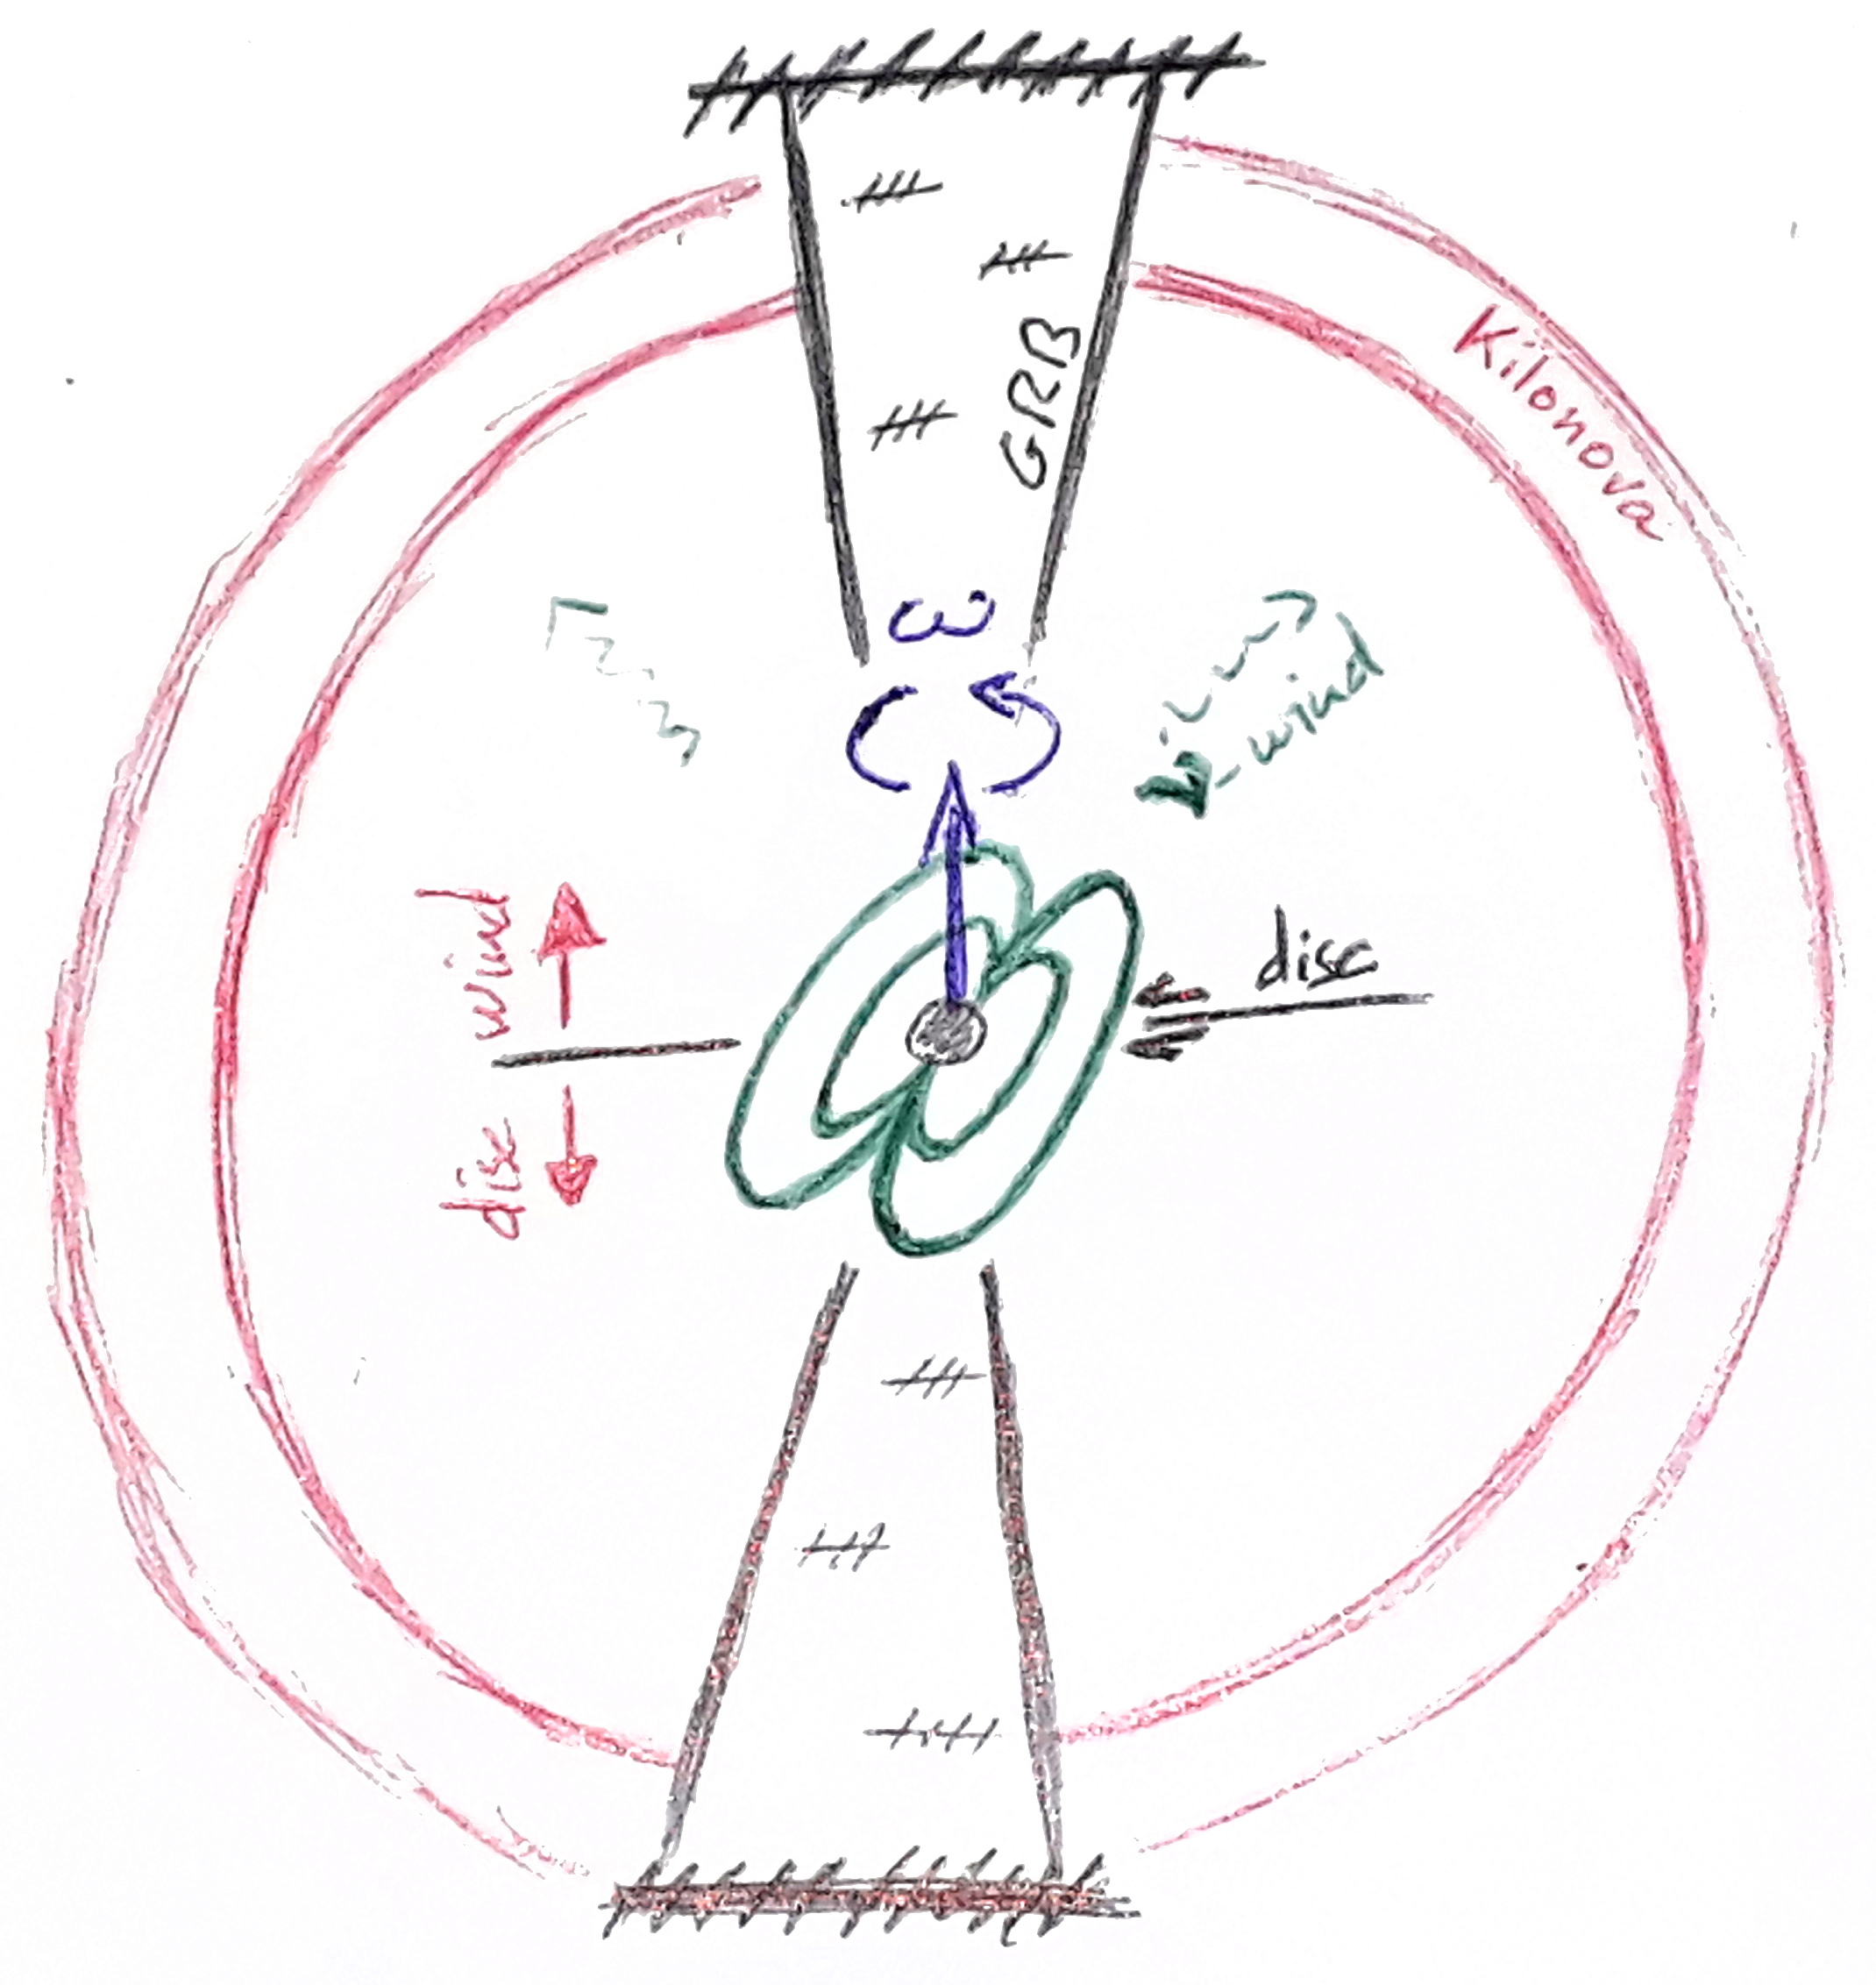
\includegraphics[width=7cm]{Figures/sketch_GRB_kilonova.jpg}}
%\vspace*{-0.4cm}
\end{figure}

\section{Gamma-ray bursts}

Short \grbs are intense non-repeating flares of approximately $10^{51}$ ergs released as gamma-rays over less than two seconds \citep{Berger2014}. With the discovery of an X-ray afterglow by \citet{Gehrels2005} came the identification of the host galaxy of a short \grb and the confirmation of their cosmological origin. They have long been thought to be powered by the accretion of a massive remnant disc onto the compact object formed after a \ns-\ns/\bh-\ns merger \citep{Eichler1989}. The interplay between accretion and rapid rotation of the central engine can drive a collimated ultra-relativistic outflow or a jet \citep{Piran2005}. Relativistically beamed gamma-ray emission arises from energy dissipation via internal shocks within the jet \citep{Rees1992} and external shocks with circumburst material generate the aforementioned afterglow \citep{Kumar2015}. In France, \grbs lie at the core of the theoretical models developed by Fr\'ed\'eric Daigne, Robert Mochkovitch and their collaborators in the ASTHUP team but also by Guillaume Dubus, Beno\^it Cerutti, Guy Pelletier and the Sherpas group at IPAG and by Thierry Foglizzo and his collaborators at CEA/Irfu. They are the prime targets of the \textit{SVOM} mission and many people in France are devoted to their observational study, at IRAP for instance. Furthermore, mid-January 2019, a rapid follow-up of the \grb \textit{GRB-190114C} detected by Swift/BAT led to the first sub-TeV detection of a \grb from the ground thanks to the MAGIC Cherenkov telescopes. Although the origin and properties of this \grb are still unclear, it opens the possibility of ground-based gamma-ray Astronomy with the upcoming CTA (Cherenkov Telescope Array) France is involved in.\\

The accretion disc plays a key role in the accretion/ejection mechanism which connects the different components and eventually produces the electromagnetic counterpart we observe. Due to its connections with the jet responsible for the short \grb, I want to address the following main questions:
\begin{enumerate}[itemsep=0mm]
\item under which conditions a disc is formed and which are its initial properties?
\item how do disc outflows develop and to what extent do they constrain the lateral expansion of the jet?
\end{enumerate}

\subsection{Accretion discs formed by \ns tidal disruption}

When two \nss merge, a fraction of the material is tidally disrupted and can form a disc \citep{Baiotti2017}, while magnetic field rearrangement occurs \citep{Crinquand2018}. When a \ns merges with a \bh, the situation is different: a disc can only be formed provided the tidal disruption of the \ns occurs before the innermost stable circular orbit (ISCO), a critical distance below which the amount of angular momentum is too low to maintain a circular orbit. The constrain set by the presence of the ISCO has been shown to be very stringent. In Figure\,\ref{fig:disc_condition}, I represented in fully opaque green the zone where the tidal disruption of a 1.4\msun \ns would lead to the formation of a disc \citep[based on arguments inspired from][]{Foucart2012}. This preliminary approach seems to indicate that only mergers of \nss with low mass \bhs ($\lesssim$5\msun) could lead to the formation of a disc but the result depends strongly on the \bh spin and the redistribution of angular momentum between the ejected material and the inspiralling \ns. Numerical simulations are required to evaluate the disc properties and its dependencies on the different parameters.\\

I will make use of the angular momentum preserving scheme I developed for \texttt{MPI-AMRVAC} to monitor the disc formation in \ns-\ns/\bh-\ns mergers with numerical simulations. To avoid any non-physical variations of the total angular momentum, I implemented a new way to solve the conservation of linear momentum which guarantees angular momentum conservation to machine precision \citep{ElMellah2019}. It assures that the obtained discs have radial extensions physically accurate. I would be able to make use of the post-Newtonian formalism developed by Luc Blanchet, Guillaume Faye and their collaborators in the GreCo team at IAP to significantly speed up the simulations. Indeed, the full general relativistic treatment of the dynamics requires costly root-finding algorithms we could bypass thanks to a post-Newtonian formulation of the equations. Because computationally-demanding three-dimensional simulations will be required to evaluate the impact of the line-of-sight on the observables, such a speed-up is of prime importance.\\

\begin{figure}[!h]
\vspace*{-0.2cm}
\floatbox[{\capbeside\thisfloatsetup{capbesideposition={right,center},capbesidewidth=6cm}}]{figure}[\FBwidth]
{\caption{Ratio of the tidal disruption radius of a 1.4\msun \ns by the radius of the ISCO of a non-rotating \bh, as a function of the mass of the \bh. The green shaded region shows the estimated tidal disruption radius for a \ns radius between 9km (lower limit, high compacity, soft equation-of-state) and 15km (upper limit, low compacity, stiff equation-of-state). The tidal disruption radius needs to be larger than the ISCO radius to form a disc (fully opaque green shaded region).}\label{fig:disc_condition}}
{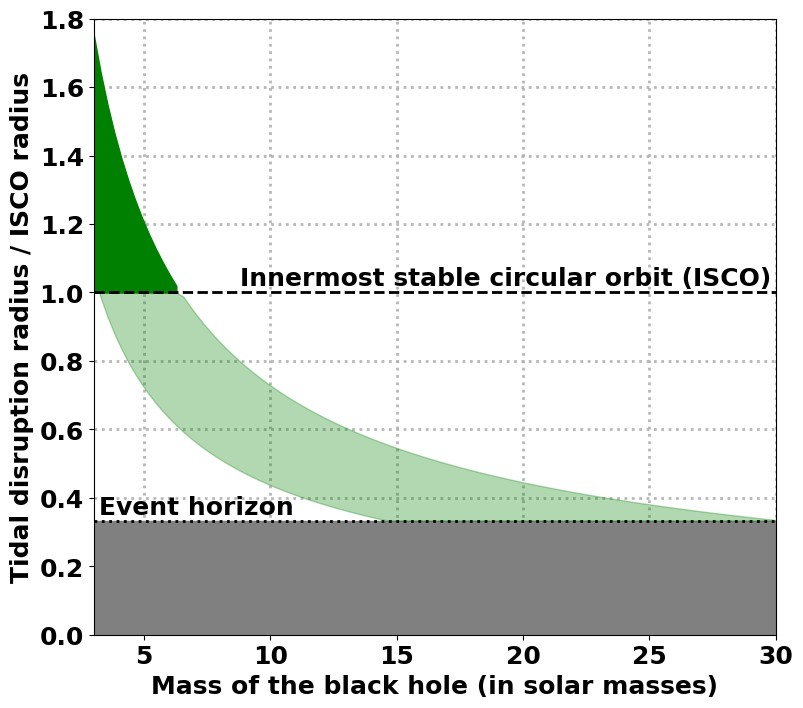
\includegraphics[width=9cm]{Figures/tidal_disruption_radius.png}}
%\vspace*{-0.4cm}
\end{figure}

\subsection{Disc accretion / ejection and jet collimation}
\label{sec:acc-ej}

Beyond the question of the structure of the disc, it is necessary to understand how the surroundings (kilonova and jet) can be impacted by the disc, both through disc outflow and radiation. Since the heating rate of the kilonova due to fall-back accretion \citep{Rosswog2007} can be of the same orders of magnitude as radioactive decay or magnetic heating (see sections\,\ref{sec:nucleo} and \ref{sec:spin} respectively), the interpretation of the kilonova light curves observed after a merger will require an accurate understanding of this connection .\\

During the first seconds following the merger, when the disc is a proficient source of neutrinos, disc outflows can rival or even dominate the dynamical ejecta \ie the mass ejected from the contact interface between the colliding \ns. Although physical differences exist between neutrinos and photons, the numerical treatment of neutrinos transport share many common points with the aforementioned radiative transfer problem. Simulations of neutrino-driven winds would quantify the amount of mass and energy reinjected in the kilonova by the disc outflow. As neutrino-cooling becomes inefficient, the disc transitions to a geometrically thick regime and the wind becomes richer in heavy elements such as lanthanides whose high opacity changes the emission properties. The hot surface of the disc acts like a stellar photosphere and the wind launching mechanism is similar to the one of line-driven winds of massive stars \citep{Castor1975}, a topic I extensively studied for the last three years, using numerical techniques such as periodic long characteristics in Cartesian slabs and effective acceleration inhibition distance \citep{ElMellah2018}. I will extend these methods to model the specificities of this type of discs.\\

In such a highly optically thick disc, the coupling between matter and radiation must be accounted for. In order to do so, we developed an implicit multi-grid solver with Jannis Teunissen (CWI Amsterdam) and Nicolas Moens, a graduate student I co-supervise with Jon Sundqvist in KU Leuven. It is based on a flux-limited diffusion approach which represents a computationally-affordable method to solve the radiative transfer equation.\\

Finally, once the disc outflow has been constrained, its connection with the jet could be studied without prescribing ad hoc launching conditions. It has been suggested that the lateral expansion of the jet is initially limited by the denser disc wind (see Figure\,\ref{fig:disc-jet_Sasha}). Using \texttt{MPI-AMRVAC} with post-Newtonian prescriptions, I could study the modalities of this confinement in high-resolution three-dimensional simulations. On this occasion, I would actively collaborate with Martin Lemoine (IAP) whose work on collisionless relativistic shocks in the jet produced by non-stationary launching conditions \citep{Pelletier2017} would benefit from these numerical simulations. \\

\begin{figure}[!h]
\vspace*{-0.2cm}
\floatbox[{\capbeside\thisfloatsetup{capbesideposition={right,center},capbesidewidth=5.5cm}}]{figure}[\FBwidth]
{\caption{Density and magnetic field contours from a simulation by \citet{Kathirgamaraju2019} where a low-density relativistic jet is launched from the compact object at the origin. The lengths are scaled with gravitational radii and $\rho_0\sim7\cdot 10^{16}$g$\cdot$cm$^{-3}$. These simulations were performed from a prescribed torus as initial conditions.}\label{fig:disc-jet_Sasha}}
{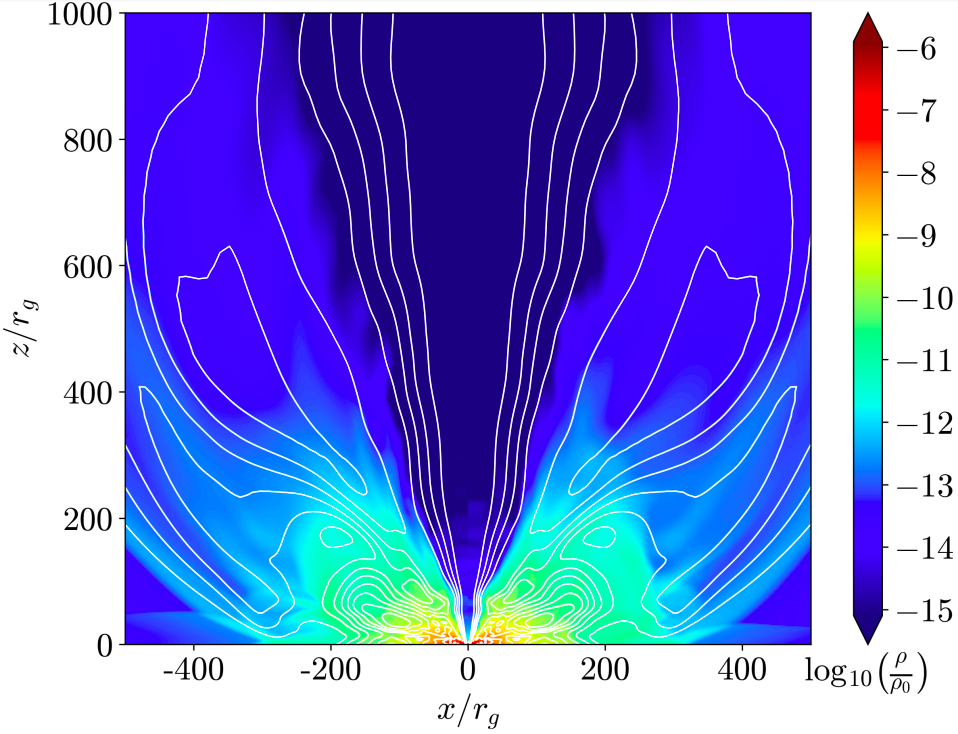
\includegraphics[width=10cm]{Figures/disc-jet_Sasha.png}}
\end{figure}

\vspace*{-0.4cm}

\section{Kilonovae}

Kilonovae are week-long supernovae-like transients found in association with short \grbs, with a spectral peak ranging from near infrared to optical and a peak luminosity at 10$^{40-41}$erg$\cdot$s$^{-1}$ reached after a few days \citep{Tanaka2016,Metzger2017}. They are thought to be produced by neutron-rich material ejected during a \ns-\ns/\bh-\ns merger: as the mildly relativistic cocoon expands, it is heated by radioactive decay \citep{Li1998} but also by fall-back accretion onto the central body (see section\,\ref{sec:acc-ej}) and possibly by a millisecond magnetar formed by the merger \citep{Yu2013}.\\

The relative contribution of these mechanisms will be a central problem to interpret the kilonovae light curves observed in coincidence with \gw signals from \ns-\ns mergers, which will lead the community to address the following questions:

\begin{enumerate}[itemsep=0mm]
\item How neutron-rich are the different components of the ejecta?
\item How can the rotational energy of a fastly rotating magnetar remnant be transferred to the ejecta?
\end{enumerate}

\subsection{A site for nucleosynthesis of neutron-rich elements}
\label{sec:nucleo}

Kilonovae have long been suspected to be the main site for the nucleosynthesis of the heaviest elements \citep{Lattimer1974}, along with core-collapse supernovae \citep{MacFadyen1999}. Due to their dense neutron-rich content (\ie low electron fraction), kilonovae can be the stage of rapid neutron-capture by seed nuclei like Iron, the so-called "r-process". The yield of this nucleosynthesis and the associated heating of the kilonova can be derived from nuclear reaction networks \citep{Metzger2010} and the electron fraction, with higher yields for lower electron fractions. However, the electron fraction can only be deduced once we properly account for neutrino-irradiation: neutrino absorption reactions on nucleons increase the electron fraction of the material and might inhibit the formation of lanthanides. Since the opacity of lanthanides can quickly dominate and determine the properties of a kilonova light curve, we need to figure out how neutrinos interact with the different components during a \ns-\ns/\bh-\ns merger.\\

Computationally efficient methods to solve neutrino transport in the context of core-collapse supernovae have been developed by members of the LUTh in Meudon \citep{Peres2011,Peres2013}. I propose to extend this treatment to \ns-\ns/\bh-\ns mergers and implement it in a form suitable to be used in conjunction with \texttt{MPI-AMRVAC}. During my postdoctoral years, I have worked on different schemes to solve the radiative transfer equations: methods inspired from long characteristics with Jon Sundqvist, flux-limited diffusion and an alternating directional implicit scheme with Nicolas Moens and multi-grid solvers with Jannis Teunissen. I will adapt these methods to neutrino transport. Coupling the micro-Physics to the flow dynamics has become an absolute requirement to improve our understanding of these high-temperature environments. 

\subsection{Spinning down of a magnetar remnant}
\label{sec:spin}

Extraction of the huge rotational energy contained in a millisecond magnetar (\ie with a magnetic field strength above 10$^{14}$G) via electromagnetic torques might significantly enhance the electromagnetic emission from \ns-\ns mergers. It could be a major source of heating for the kilonova, provided it can sustain a high spinning down luminosity for long enough (see Figure\,\ref{fig:spinning_down}). The modalities of the coupling between the plasma and the magnetosphere depend strongly on the relative extension of the magnetosphere with respect to the corotation radius, the radius at which the period of a Keplerian orbit matches the \ns spin period \citep[see \eg the propeller effect described in][]{Bozzo2008}. \\

I am currently working, in collaboration with Zakaria Meliani (LUTh), on \mhd setups to compute torques applied to \nss in X-ray binaries. Thanks to the radially stretched meshes I implemented during my PhD, we could adapt these setups to kilonovae and characterize the impact of the interaction with the spinning down magnetosphere on the dynamics of the flow. \\

This work would bring key information to shed unprecedented light on another topic of interest of contemporary Astrophysics: the internal structure of \nss and their equation-of-state (\eos). When a \ns-\ns merger occurs, three different types of remnants can be formed, from the lighter to the heavier: a stable \ns, a supramassive \ns sustained by its solid body rotation, or a body immediately collapsing into a \bh (for simplicity, I include hypermassive \ns in this last case). While a stable magnetar can participate indefinitely in the heating of the kilonova (although at lower levels as time goes by), a supramassive \ns will collapse into a \bh once it spins down below a certain threshold: in this case, only a fraction of the rotational energy can be extracted before the \ns collapses. The possibility of a short or long-lived \ns remnant could not be ruled out in the \gw signal of the 2017 double \ns merger.\\

In Figure\,\ref{fig:spinning_down} is represented the simplified spinning-down luminosity of an aligned rotating dipole \citep{Spitkovsky2006,Philippov2014}. Its plateau value scales as the square of the \ns magnetic field but the spinning down time scales as the revert of the square of the magnetic field: a higher magnetic field starts at a higher luminosity level but quickly decreases below the plateau level a lower magnetic field can sustain for a longer period of time. The premature endings of the curves for a supramassive \ns (green lines) indicates the collapse of the \ns into a \bh, assuming a \ns \eos which leads to a collapse time similar to the spinning down time for a 2.4M$_{\odot}$ \ns \citep[based on][]{Metzger2015}.\\

These four illustrative limit cases could be explored in much more detail with full three-dimensional \mhd numerical simulations. I am willing to make use of the extensive numerical expertise I have acquired in this domain over the last years to capture these different regimes and evaluate the impacts on the light curve of the kilonova. The effect of the collapse time, tidally linked to the \eos of the condensed matter in \ns interior, could also be investigated. Once confronted to a large sample of observed double \ns mergers, numerical results would set stringent constrains on the \ns \eos.\\

\begin{figure}[!h]
\vspace*{-0.2cm}
\floatbox[{\capbeside\thisfloatsetup{capbesideposition={right,center},capbesidewidth=6cm}}]{figure}[\FBwidth]
{\caption{Rates of \ns rotational energy decay as a function of time. Different \ns magnetic field strengths and masses are considered, and standard parameters taken from \citet{Metzger2017} are used. While a 2M$_{\odot}$ \ns does not need centrifugal support to avoid collapsing into a \bh, a 2.4M$_{\odot}$ \ns might qualify as a supramassive \ns (depending on the \eos) and collapse once it has evacuated too much rotational energy (green dots). See text for more details.}\label{fig:spinning_down}}
{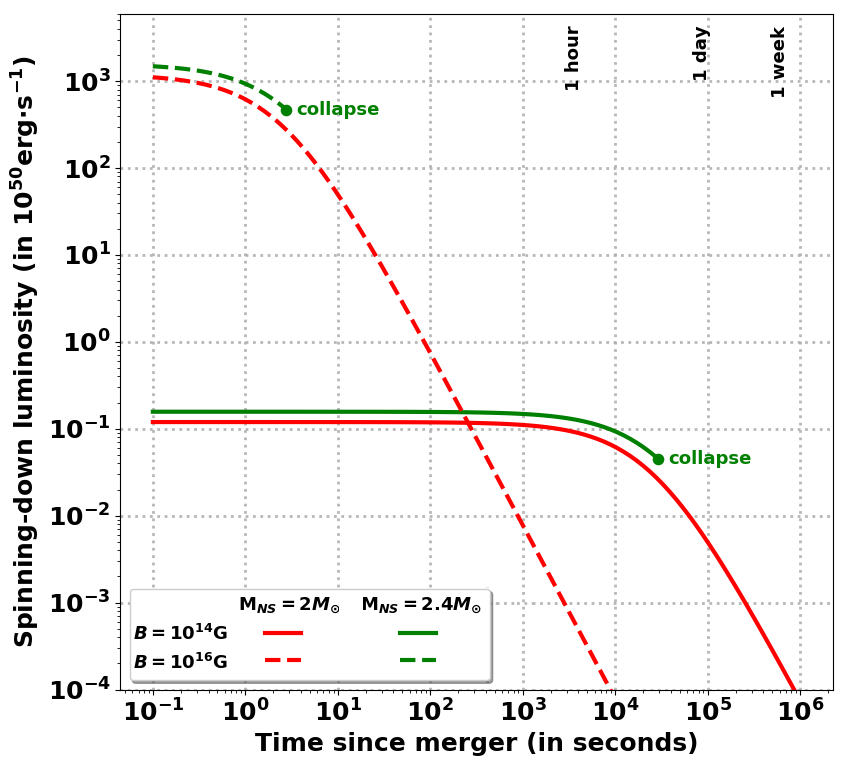
\includegraphics[width=10cm]{Figures/spinning-down_luminosity.png}}
%\vspace*{-0.4cm}
\end{figure}

\newpage

\section*{Conclusion}

The properties of the electromagnetic counterparts detected with the \gw signal of 2017 are still puzzling in many aspects. Was the blue color of the kilonova due to the formation of a long-lived \ns whose flux of neutrinos could have inhibited lanthanide nucleosynthesis? Was its high luminosity due to the heating by fall-back accretion onto a \bh formed by the merger of the two \nss? Or by magnetic heating from a strongly magnetized remnant \ns? Was the short \grb intrinsically fainter due to the absence of \bh formation \citep{Murguia-Berthier2017a}? Or was it an ultra-relativistic jet seen off-axis? \\

Many unanswered questions remain and more are to be expected in the next years. The interpretation of the plethora of kilonovae light curves and short \grbs to come requires a better understanding of the Physics at stake now that new constrains are set by the concomitant \gw and \grb observations. I am willing to take part in this collective effort in the ASTHUP team at IAP. I have no doubt I can trigger new collaborations with the GreCo team to take advantage of their expertise in gravitational theory and foster renewed partnerships with the ASTHUP team, along with the neighboring LUTh at the Observatory of Meudon. On the long term, the X-IFU instrument aboard the Athena satellite will provide high-resolution X-ray spectra to characterize the ionization properties of the material surrounding the compact remnant after a \ns-\ns/\bh-\ns merger. It will bring new insights on the deposition of energy in the ejecta, of direct interest to be compared with predictions from numerical simulations.\\

%Efforts at the LUTh by Zakaria Meliani have been made to make \texttt{MPI-AMRVAC} solve the Einstein equations and compute dynamical non-analytic metrics. The proximity of LUTh at Meudon and IAP in Paris is a unique chance since they both host world-leading experts in general relativity and alternative theories of gravity whose knowledge is of tremendous importance to design the numerical schemes appropriate to perform such a computation. In the longer term, coupling tools like the spectral solver Kadath developed by Philippe Grandcl\'{e}ment (LUTh) to \texttt{MPI-AMRVAC} would lead to a brand new family of codes solving the dynamics of the flow and the metrics all together, a decisive asset in the relativistic environment of a compact object merger. On the other hand, the models of \grb designed by Fr\'{e}d\'{e}ric Daigne provide a firm semi-analytical bedrock to build upon. These models can make accurate predictions for simplified geometries or in asymptotic regimes which serve to validate numerical setups before running jobs on high performance computing facilities.

%I am willing to take part in this collective effort at LUTh and to bring a numerical expertise suitable to the problems tackled by its members. As my supervision record indicates, I would try to attract excellent Master and PhD candidates to support this effort. Thanks to the Pegasus Marie Sk\l{}odowska-Curie grant I received in 2017, I am also in an ideal position to apply for ERC grants in the following years, in an attempt to provide the necessary momentum to the field of kilonovae and short \grbs in France.




%\phantom{\cite{ElMellah2016a,ElMellah2018a,Xia2017,Rappaport:2012wi,Rappaport2013,SanchisOjeda:2014ww}}
%%\subsubsection*{References}
%\vspace*{0.6cm}
\setlength\bibitemsep{0pt}
%%\scriptsize
%\bibliographystyle{ieeetr}
%\bibliography{/Users/Ileyk/Documents/Bibtex/Hubble_fellowship_no_url}

%\settoggle{bbx:url}{false}
%\settoggle{bbx:doi}{false}
%\settoggle{bbx:eprint}{false}
%\bibliographystyle{ieeetr}
%\nocite{MEMSnet,wilde,markey}
\printbibliography[heading=none,title={},omitnumbers=true]


\end{document}
%%%%%%%%%%%%%%%%%  Fin du fichier Latex  %%%%%%%%%%%%%%%%%%%%%%%%%%%%%%

